%%%%%%%%%%%%%%%%%%%%%%%%%%%%%%%%%%%%%%%%%%%%%%%%%%%%%%%%%%%%%%%%%%
%%                                                              %%
%% Template f�r Studien-, Diplom-, Bachelor- und Masterarbeiten %%
%%                 am Lehrstuhl ISE der CAU Kiel                %%
%%                                                              %%
%%                              17.10.2006                      %%
%%                                                              %%
%%%%%%%%%%%%%%%%%%%%%%%%%%%%%%%%%%%%%%%%%%%%%%%%%%%%%%%%%%%%%%%%%%
 
%% Stellen, an denen noch Daten eingetragen werden m�ssen,
%% sind mit ** gekennzeichnet.

%% Gr��e: A4, doppelseitig 
\documentclass[twoside,a4paper,BCOR1.0cm]{scrbook}

\usepackage{ifpdf}

\usepackage{ae,aecompl}
\usepackage[latin1]{inputenc} %% unter Linux/Unix "ansinew" evtl. durch "latin1" ersetzen
\usepackage{amsthm}
\usepackage{amsfonts}
\newtheorem{definition}{Definition}
%%\usepackage{ngerman}
%%\usepackage{url}

%% Falls PicTeX-Grafiken (z.B. aus XFig) eingebunden werden sollen
%%\usepackage{pictexwd}

%% einige mathematische Symbole (falls ben�tigt)
%%\usepackage{stmaryrd}
\usepackage[intlimits]{amsmath}
%%\usepackage{amssymb}

%% f�r listings-Umgebungen und Algorithmen
\usepackage{algorithm}
\usepackage{algpseudocode}
\usepackage{listings}

%%\renewcommand{\listalgorithmname}{Listingsverzeichnis} 

%% Literatur-Verzeichnis
\usepackage{natbib}
\bibpunct{[}{]}{;}{a}{,}{,}

\ifpdf
  % f�r Grafiken
  \usepackage[pdftex]{graphicx}
  
  % Verweise in PDF
  \usepackage[pdftex,plainpages=false]{hyperref}
  \pdfcompresslevel=9  

  % Metadaten des Dokuments
  \hypersetup{%
    a4paper,
    pdftitle = {** Hier den Titel eintragen **},
    pdfsubject = {** Hier eine Beschreibung eintragen **},
    pdfkeywords = {** Hier Schlagw�rter eintragen **},
    pdfauthor = {** Hier den Namen des Autors eintragen **},
    % pdfpagemode = None, UseThumbs, UseOutlines, FullScreen,
    % pdfstartpage = ,
    % pdfstartview = 
  }
\else
  \usepackage[plainpages=false]{hyperref}
  \usepackage{graphicx}
\fi    
\usepackage{todonotes}
\usepackage{tikz}
\usetikzlibrary{arrows,automata,positioning}


\setlength{\parindent}{0cm}

\begin{document}
\ifpdf
  \DeclareGraphicsExtensions{.jpg, .pdf, .mps, .png}
\else
  \DeclareGraphicsExtensions{.eps}
\fi

\renewcommand{\textfraction}{0.1}

%%%%%%%%%%%%%%%%%%%%%%%%%%%%%%%%%%%%%%%%%%%%%%%%%%%%%%%%%%%%%%%%%%
%%                                                              %%
%%                          Titelseite                          %%
%%                                                              %%
%%%%%%%%%%%%%%%%%%%%%%%%%%%%%%%%%%%%%%%%%%%%%%%%%%%%%%%%%%%%%%%%%%

\pagestyle{empty}

\begin{center}
{\huge \it **[Studien|Diplom|Bachelor|Master]arbeit**}

\vspace{2cm}

{\Large \bf ** Titel der Arbeit **}

\vspace{2.25cm}

%%\includegraphics[height=4cm]{CAU-Siegel}

\vspace{2.25cm}

{\large 
Christian-Albrechts-Universit�t zu Kiel \\
Institut f�r Informatik  \\
Lehrstuhl Technologie der Informationssysteme
}

\end{center}

\vspace{2cm}

\begin{tabular}{ll}
angefertigt von:             & {\bf ** eigener Name **} \\
betreuender Hochschullehrer: & ** Name des betreuenden Hochschullehrers ** \\%
%                              z.B. Prof. Dr. rer. nat. habil. Bernhard Thalheim 
%                              oder Prof. Dr. rer. nat. habil. Hans-Joachim Klein
Betreuer:                    & ** Name des Betreuers ** 
\end{tabular}

\vspace{1cm}

\begin{center}
Kiel, ** Datum der Abgabe **
\end{center}


\cleardoublepage

%%%%%%%%%%%%%%%%%%%%%%%%%%%%%%%%%%%%%%%%%%%%%%%%%%%%%%%%%%%%%%%%%%
%%                                                              %%
%%                      Aufgabenstellung                        %%
%%                                                              %%
%%%%%%%%%%%%%%%%%%%%%%%%%%%%%%%%%%%%%%%%%%%%%%%%%%%%%%%%%%%%%%%%%%

% \pagestyle{plain}
% \chapter*{Aufgabe}

% \begin{tabular}{ll}
% {\bf Name, Vorname: }               & ** Name, Vorname **                            \\
% {\bf Immatrikulations-Nr: }         & ** Immatrikulations-Nr **                      \\
% {\bf Studiengang: }                 & ** Studiengang **                              \\
%                                     &                                                \\
% {\bf betreuender Hochschullehrer: } & ** Name des Hochschullehrers **   \\
% {\bf Betreuer: }                    & ** Name des Betreuers **                       \\
% {\bf Institut: }                    & Institut f�r Informatik  \\
% {\bf Arbeitsgruppe: }               & Technologie der Informationssysteme            \\
%                                     &                                                \\
% {\bf Beginn am: }                   & ** Datum des Beginns **                        \\
% {\bf Einzureichen bis: }            & ** Abgabetermin **                           
% \end{tabular}

% \vspace{1cm}

% {\bf Aufgabenstellung:}

% \vspace{0.5cm}

% ** Text der Aufgabenstellung **

% \pagenumbering{roman}
% \setcounter{page}{1}
% \cleardoublepage

%%%%%%%%%%%%%%%%%%%%%%%%%%%%%%%%%%%%%%%%%%%%%%%%%%%%%%%%%%%%%%%%%%
%%                                                              %%
%%                Selbstst�ndigkeitserkl�rung                   %%
%%                                                              %%
%%%%%%%%%%%%%%%%%%%%%%%%%%%%%%%%%%%%%%%%%%%%%%%%%%%%%%%%%%%%%%%%%%

\chapter*{Selbstst�ndigkeitserkl�rung}

\vspace{1.5cm}

Ich erkl�re hiermit, dass ich die vorliegende Arbeit selbstst�ndig und nur unter Verwendung der angegebenen Literatur und Hilfsmittel angefertigt habe.

\vspace{2cm}
............................................................... \\
** eigener Name **

\thispagestyle{plain}
\cleardoublepage

%%%%%%%%%%%%%%%%%%%%%%%%%%%%%%%%%%%%%%%%%%%%%%%%%%%%%%%%%%%%%%%%%%
%%                                                              %%
%%                     Inhaltsverzeichnis                       %%
%%                                                              %%
%%%%%%%%%%%%%%%%%%%%%%%%%%%%%%%%%%%%%%%%%%%%%%%%%%%%%%%%%%%%%%%%%%

\tableofcontents

\cleardoublepage

%%%%%%%%%%%%%%%%%%%%%%%%%%%%%%%%%%%%%%%%%%%%%%%%%%%%%%%%%%%%%%%%%%
%%                                                              %%
%%                     Abbildungsverzeichnis                    %%
%%                                                              %%
%%%%%%%%%%%%%%%%%%%%%%%%%%%%%%%%%%%%%%%%%%%%%%%%%%%%%%%%%%%%%%%%%%

\listoffigures

\cleardoublepage

%%%%%%%%%%%%%%%%%%%%%%%%%%%%%%%%%%%%%%%%%%%%%%%%%%%%%%%%%%%%%%%%%%
%%                                                              %%
%%                     Tabellenverzeichnis                      %%
%%                                                              %%
%%%%%%%%%%%%%%%%%%%%%%%%%%%%%%%%%%%%%%%%%%%%%%%%%%%%%%%%%%%%%%%%%%

\listoftables

\cleardoublepage

%%%%%%%%%%%%%%%%%%%%%%%%%%%%%%%%%%%%%%%%%%%%%%%%%%%%%%%%%%%%%%%%%%
%%                                                              %%
%%                   Algorithmenverzeichnis                     %%
%%                                                              %%
%%%%%%%%%%%%%%%%%%%%%%%%%%%%%%%%%%%%%%%%%%%%%%%%%%%%%%%%%%%%%%%%%%

\listofalgorithms

\cleardoublepage

%%%%%%%%%%%%%%%%%%%%%%%%%%%%%%%%%%%%%%%%%%%%%%%%%%%%%%%%%%%%%%%%%%
%%                                                              %%
%%              Liste der verwendeten Abk�rzungen               %%
%%                                                              %%
%%%%%%%%%%%%%%%%%%%%%%%%%%%%%%%%%%%%%%%%%%%%%%%%%%%%%%%%%%%%%%%%%%

\chapter*{Abk�rzungen}


\cleardoublepage

%%%%%%%%%%%%%%%%%%%%%%%%%%%%%%%%%%%%%%%%%%%%%%%%%%%%%%%%%%%%%%%%%%
%%                                                              %%
%%                       Text der Arbeit                        %%
%%                                                              %%
%%%%%%%%%%%%%%%%%%%%%%%%%%%%%%%%%%%%%%%%%%%%%%%%%%%%%%%%%%%%%%%%%%

\chapter*{Abstract}
\cleardoublepage

\pagestyle{headings}
\pagenumbering{arabic}
\setcounter{page}{1}

\chapter{Introduction}

\section{Related Work}
\section{Contributions}
\section{Overview}

%%purpose of a qa system why did I choose Askbot? 
%%how I'm getting ratings for the items
%discuss qa system, rating system, tagging system, item based, svd based, bringing it all together, display recommendations on a website
\chapter{Concepts}
\section{Question Answer System}
%explain the function and idea of a qa system, explain askbot, explain why you choosed askbot and how to integrate it.
\section{Rating System}
%explain the idea behind the implicit rating system, describe the google news approach, explain the changes that where made and why.

%%definition finite automata, deterministic finite automata 
%%why start with finite automata why create deterministic finite automata and how
\newpage
\section{Tagging}
The purpose of tagging is to find one or more keywords for a text that describe the content.
For the context of economics the \emph{STW Thesaurus for Economics} includes\todo{check number of labels and add a source}16000 labels which can be used to match words from a text and provide therefore a good tagging base.
However the \emph{STW Thesaurus for Economics} only includes the basic form of the words.
Therefore a normal test for equal is not sufficient enough.
For example a word that is used in it's plural form in a text would return false on a test for equal and would therefore not be a candidate as a tag for the text.
So, the challenge for this tagging process is to find the correct words in the \emph{STW Thesaurus for Economics} even if they are in a different form then the corresponding words from the text.
One possible solution for such a task is to reduce each word from the text to its stem. This is usually done by using predefined rules on the words. 
A rule is usually a combination of the minimum number of letters in a word, plus the suffix that should be changed, an arrow and the replacement for the suffix. More advanced algorithms might also use rules for prefix reduction and detecting irregular changes of the stem.
For example a predefined rule might be '3+ies' $\rightarrow$ 'y'. So, the word \emph{libraries} would be reduced to \emph{library}.
Thus it is important that the stemming algorithm has all necessary rules for each supported language.\todo{reason why I didn't use stemming add source for example A Fast and Simple Stemming Algorithm for German words.}
Another possible solution for the problem is to calculate the differences between the words from the text and the words from the tagging base and use the words from the tagging base as tags if they aren't too different from the original word in the text.
This creates the need for a metric that indicates the difference or distance between two words.
A practical metric for such a task is the \emph{levenshtein distance}.
\subsection{Levenshtein Distance}

The \emph{levenshtein distance} calculates the minimum numbers of substitutions, insertions and deletions that are needed to change one word into another.
Therefore it returns zero if the words are equal and adds one to the result if it has to perform a substitution an insertion or a deletion of a letter compare algorithm ~\ref{alg:levDist}.
\todo{find better solution to move 'if'}
  $levDist_{a,b}(i,j) = $
  \begin{cases}
    max(i,j) \quad \quad \quad \quad \quad \quad \quad \quad \quad \quad \quad \quad \quad \quad \text{if min(i,j) = 0} \\
    min \begin{cases}
        levDist_{a,b}(i-1, j)+1 \\
        levDist_{a,b}(i, j-1)+1 & \text{else}\\
        levDist_{a,b}(i-1, j-1) + [a_i \neq b_i] 
      \end{cases}
  \end{cases}\\
This can be directly translated into a recursive algorithm. 
\begin{algorithm}
  \caption{Recursive Levenshtein Distance Algorithm}\label{alg:levDist}
  \begin{algorithmic}[1]
    \Procedure{LevenshteinDistance}{$s: String, t: String$}
    \State $lenS\gets length(s)$
    \If{lenS = 0}
      \State \textbf{return} $lenT$
    \EndIf
    \If{lenT = 0}
      \State \textbf{return} $lenS$
    \EndIf

    \If{s[lenS-1] = t[lenT-1]}\Comment{test if last characters of the strings match}
      \State $cost\gets 0$
    \Else
      \State $cost\gets 1$
    \EndIf

    \State \textbf{return} minimum of\par
    $LevenshteinDistance(s[0..lenS-1], t) +1,$\par
    $LevenshteinDistance(s, t[0..lenT-1) +1,$\par
    $LevenshteinDistance(s[0..lenS-1], t[0..lenT-1]) + cost)$

    \EndProcedure
  \end{algorithmic}
\end{algorithm}



However the direct implementation of the \emph{levenshtein distance algorithm} has a complexity of O(something). Therefore it is a good utility to better understand the \emph{levenshtein distance} in general, but it is not feasible for a software that should work in production mode. 
\subsection{Optimized Levenshtein distance algorithm}
%definitions
\begin{definition}[Non Deterministic Finite Automata]
  A finite automata is a tupel of the form $FA = (Q, \Sigma, q_0, \Delta, F)$. 
  Q is the set of the states. $\Sigma$ is the set of the input alphabet. $q_0 \in Q$ is the initial state and $F \subset Q$ is a subset that contains the final states. $\Delta$ is a relation of the form $\Delta \subset Q \times \Sigma \times Q$. FA is called finite exactly when $Q$ is finite. Furthermore $\Sigma^*$ is the set of words over $\Sigma$ and $\epsilon$ is the empty word.
\end{definition}
\begin{definition}[Deterministic Finite Automata]
  FA is deterministic if for all $p \in Q$ and all $a \in \Sigma$ exists exactly one state $q \in Q$ with $(p, a, q) \in \Delta$. In this case $\Delta$ is written as a function $\delta : Q \times \Sigma \rightarrow Q$.
\end{definition}
\begin{definition}[Path]
  A path for FA is a series $\pi = p_0 a_1 p_1 a_2 \dots a_n p_n$, $(p_i, a_{i+1}, p_{i+1}) \in \Delta$ and $0 \leq i \leq n-1$. The length of $\pi$ is n and the label for $\beta(\pi)$ is $a_1 a_2 a_3 \dots a_n$.
\end{definition}
\begin{definition}[Path shortwriting]
  $FA: p \xrightarrow[]{\omega} q$ with $\omega \in \Sigma^*$ states, that a path $\pi$ for FA from p to q with label $\beta(\pi) = \omega$ exists.
\end{definition}
\begin{definition}[FA accepts a word]
  FA accepts $\omega \in \Sigma^*$, if and only if $p \in I, q \in F$ exists with FA: $p \xrightarrow[]{\omega} q$. For FA let $\mathcal{L}(FA)=\{\omega \in \Sigma^*$ | FA accepts $\omega\}$ be the language that FA accepts.
\end{definition}

\begin{definition}[Formal Levenshtein Distance]
  The levenshtein distance between two words $V, W \in \Sigma^*$ is the minimal number of edit operations (substitutions, deletions or insertions) that are needed to transform V into W, $d_L(V,W)$ denotes the levenshtein distance between V and W.
\end{definition}
\todo{check if I have to add source to the definitions}
\begin{definition}
  $\mathcal{L}_{Lev}(n, W)$, $n \in \mathbb{N}$ and $W \in \Sigma^*$ is the set that denotes all words $V \in \Sigma^*$ such that $d_L(W,V) \leq n$.
\end{definition}

\begin{definition}[Degree Levenshtein Automata]
  Let $W \in \Sigma^*$ and $n \in \mathbb{N}$. A finite state automaton A is a \emph{Levenshtein automaton} of degree n for W if and only if $\mathcal{L}(A) = \mathcal{L}_{Lev}(n,W)$.
\end{definition}

An optimized version of the \emph{levenshtein distance algorithm} that uses a deterministic finite automata was introduced in \emph{Fast string correction with Levenshtein automata by Schulz and Mihov}. 
The deterministic finite automata for a word $W \in \Sigma^*$ is a \emph{levenshtein automata} with degree $n \in \mathbb{N}$ with n max $d_L(W,V)$.

The purpose of the \emph{levenshtein automata} is to decide whether $d_L(W,V)$ is smaller than a specific n with $V \in \Sigma^*$.\todo{W will be changed to V and this is the levenshtein distance}
So, it is possible to decide if a word from a question is similar to a word from the \emph{STW Standard Thesaurus}, similar in the meaning it has a \emph{levenshtein distance} smaller than n.
Therefore $\Sigma$ contains the alphabet \{a,\ldots,z,A,\ldots,Z\}.
The states in Q of the \emph{levenshtein automata} denote the current position in the original word W (i) and the current \emph{levenshtein distance} between $\omega$ and W (j), with $\omega$ prefix of V.
The label of such a state is $i^j$.
Thus the initial state $q_0 \in Q$ is $0^0$.
The final states $f \in F$ are all states where i equals |W| and j is smaller than n.
The $\Delta: (Q \times \Sigma \times Q)$ is mapped as follows\todo{right translation}:\\ 
\begin{math}
(i^j, \sigma) \rightarrow \begin{cases}
  (i+1)^j & \text{if correct}\\
  (i)^{(j+1)} & \text{if insertion}\\
  (i+1)^{(j+1)} & \text{if substitution or deletion}\\
  empty & \text{if j is equal to n}
\end{cases}
\end{math}

Non Deterministic Levenshtein automata for the word \emph{test}\\
\begin{figure}[h]
  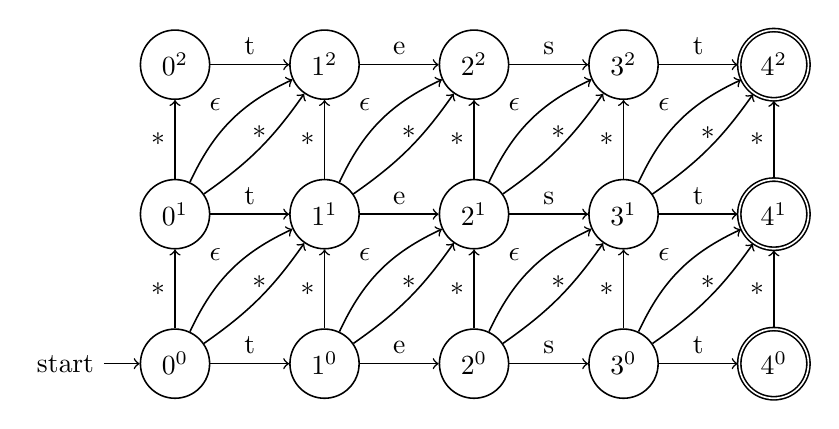
\begin{tikzpicture}[->,auto,line width=0.2mm] 
    %0,0 row
    \node[state] (q_2) {$0^2$}; 
    \node[state] (q_1) [below =of q_2] {$0^1$}; 
    \node[state,initial] (q_0) [below =of q_1] {$0^0$}; 

    %1,0 row t
    \node[state] (q_5) [right =of q_2] {$1^2$}; 
    \node[state] (q_4) [right =of q_1] {$1^1$}; 
    \node[state] (q_3) [right =of q_0] {$1^0$}; 

    %2,0 row e
    \node[state] (q_8) [right =of q_5] {$2^2$}; 
    \node[state] (q_7) [right =of q_4] {$2^1$}; 
    \node[state] (q_6) [right =of q_3] {$2^0$};

    %3,0 row s
    \node[state] (q_11) [right =of q_8] {$3^2$}; 
    \node[state] (q_10) [right =of q_7] {$3^1$}; 
    \node[state] (q_9) [right =of q_6] {$3^0$};

    %4,0 row t
    \node[state, accepting] (q_14) [right =of q_11] {$4^2$}; 
    \node[state, accepting] (q_13) [right =of q_10] {$4^1$}; 
    \node[state, accepting] (q_12) [right =of q_9] {$4^0$};

    %path deletion 0,0
    \path[->] 
    (q_0) edge node {$*$} (q_1)
    (q_1) edge node {$*$} (q_2);
    %path 0,0 -> 1,0
    \path[->] 
    %correct path
    (q_0) edge  node {t} (q_3)
    (q_1) edge  node  {t} (q_4)
    (q_2) edge  node  {t} (q_5)

    %insertion substitution
    (q_0) edge[bend right=10]  node[above,midway] {$*$} (q_4)
    (q_0) edge[bend left=20]  node  {$\epsilon$} (q_4)


    (q_1) edge[bend right=10]  node[above,midway] {$*$} (q_5)
    (q_1) edge[bend left=20]  node  {$\epsilon$} (q_5);

    %path deletion 1,0
    \path[->] 
    (q_3) edge node {$*$} (q_4)
    (q_4) edge node {$*$} (q_5);

    %path 1,0 -> 2,0
    \path[->] 
    %correct path
    (q_3) edge  node {e} (q_6)
    (q_4) edge  node  {e} (q_7)
    (q_5) edge  node  {e} (q_8)

    %insertion substitution
    (q_3) edge[bend right=10]  node[above,midway] {$*$} (q_7)
    (q_3) edge[bend left=20]  node  {$\epsilon$} (q_7)


    (q_4) edge[bend right=10]  node[above,midway] {$*$} (q_8)
    (q_4) edge[bend left=20]  node  {$\epsilon$} (q_8);


    %path deletion 2,0
    \path[->] 
    (q_6) edge node {$*$} (q_7)
    (q_7) edge node {$*$} (q_8);

    %path 1,0 -> 2,0
    \path[->] 
    %correct path
    (q_6) edge  node {s} (q_9)
    (q_7) edge  node  {s} (q_10)
    (q_8) edge  node  {s} (q_11)

    %insertion substitution
    (q_6) edge[bend right=10]  node[above,midway] {$*$} (q_10)
    (q_6) edge[bend left=20]  node  {$\epsilon$} (q_10)


    (q_7) edge[bend right=10]  node[above,midway] {$*$} (q_11)
    (q_7) edge[bend left=20]  node  {$\epsilon$} (q_11);

    %path deletion 3,0
    \path[->] 
    (q_9) edge node {$*$} (q_10)
    (q_10) edge node {$*$} (q_11);

    %path 3,0 -> 4,0
    \path[->] 
    %correct path
    (q_9) edge  node {t} (q_12)
    (q_10) edge  node  {t} (q_13)
    (q_11) edge  node  {t} (q_14)

    %insertion substitution
    (q_9) edge[bend right=10]  node[above,midway] {$*$} (q_13)
    (q_9) edge[bend left=20]  node  {$\epsilon$} (q_13)


    (q_10) edge[bend right=10]  node[above,midway] {$*$} (q_14)
    (q_10) edge[bend left=20]  node  {$\epsilon$} (q_14);

    %path deletion 3,0
    \path[->] 
    (q_12) edge node {$*$} (q_13)
    (q_13) edge node {$*$} (q_14);


  \end{tikzpicture}
  \caption{A non deterministic levenshtein automata for the word \emph{test} with degree 2}
  \label{ndla}
\end{figure}
The automata in example ~\ref{ndla} is a non deterministic levenshtein automata for the word \emph{test}.
The initial state $0^0$ is in the bottom left corner. If the automata reads a correct letter it follows the horizontal path. The star (*) indicates that any element from $\Sigma$ is accepted on this path.
A vertical path is an insertion and on a diagonal path it can be a deletion with the empty word $\epsilon$ or a substitution of the letter indicated with *. 
Therefore after reading the letter 't' the automata can be in five different states namely $0^1$, $1^2$, $1^1$, $2^2$ and $1^0$.
\todo{Problems with non deterministic automatas. How to generate a deterministic automata. example}
Evaluating a non deterministic levenshtein automata is computational complex due to the fact that there can be a large number of active states at the same time. 
Thus it is necessary to convert a non deterministic automata to a deterministic automata before using it to find tags.
The process of generating a deterministic automata with a non deterministic automata is called \emph{powerset construction}.

\subsubsection{Powerset Construction}
\todo{add source book Introduction to Automata Theory, Languages and Computation by Hopcroft, Motwani }
Given a \emph{non deterministic levenshtein automata} the construction of an equivalent \emph{deterministic levenshtein automata}: 
\begin{itemize}
  \item create $q_0'$ as a set with original $q_0$ and all states that are reachable with an $\epsilon$ path.
  \item $Q' \subseteq 2^Q$, thus all $q \in Q'$ are subsets of Q.
  \item $\delta(R,a) = \{q \in Q$ | $\exists r \in R$ with (r, a, q) $\in \Delta$ $\lor$ (r, $\epsilon$, q) $\in \Delta$ $\lor$ (r, $\epsilon$, p) and (p, a, q) $\in \Delta\}, R \subseteq Q$.
  \item F' includes all $q \in Q'$ that include $f \in F$
\end{itemize}
Therefore the new \emph{deterministic levenshtein automata} is (Q', $\Sigma$, $q_0'$, $\delta$, F').


\newpage
Deterministic Levenshtein automata example for the word test with max \emph{levenshtein distance} 1.
\todo{finish automata}
\begin{figure}[h]
  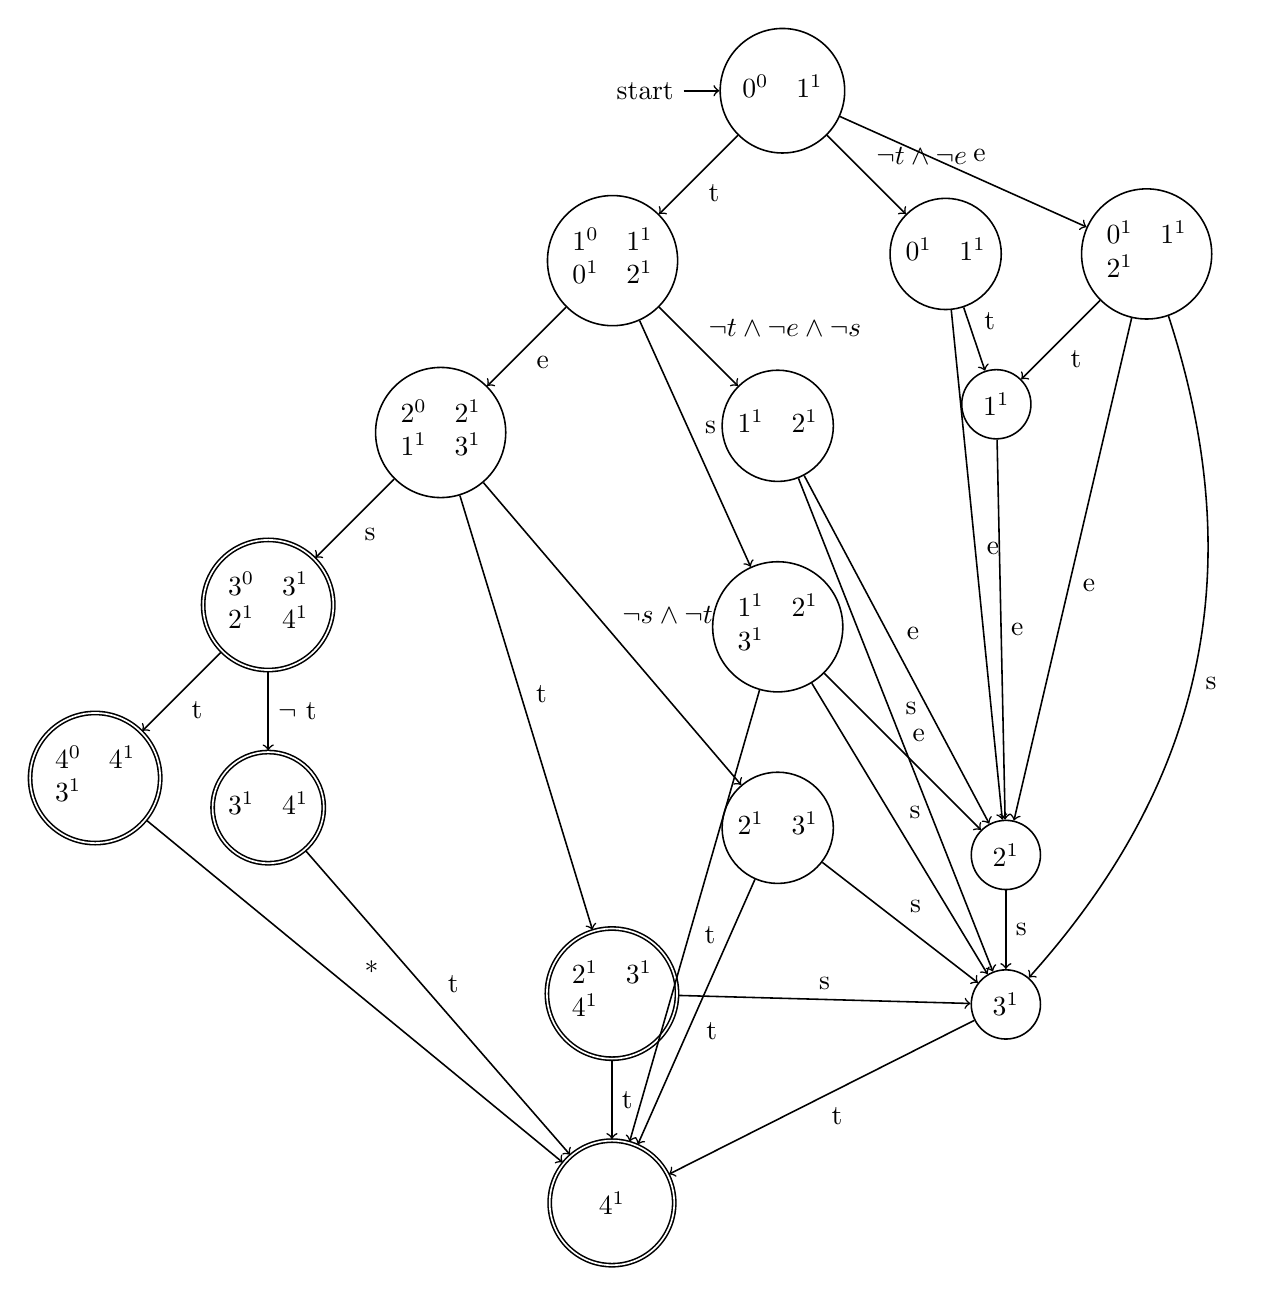
\begin{tikzpicture}[->,auto,line width=0.2mm] 
    \node[state,initial, minimum size=4.5em] (0_0-1_1) {$\begin{matrix} 0^0 & 1^1 \end{matrix}$}; 
    %correct path
     \node[state] (1_0-1_1-0_1-2_1) [below left=of 0_0-1_1] {$\begin{matrix} 1^0 & 1^1\\ 0^1 & 2^1 \end{matrix}$}; 
     \node[state] (2_0-2_1-1_1-3_1) [below left=of 1_0-1_1-0_1-2_1] {$\begin{matrix} 2^0 & 2^1\\ 1^1 & 3^1 \end{matrix}$}; 
     \node[state, accepting] (3_0-3_1-2_1-4_1) [below left=of 2_0-2_1-1_1-3_1] {$\begin{matrix} 3^0 & 3^1\\ 2^1 & 4^1 \end{matrix}$}; 

     \node[state, accepting] (4_0-4_1-3_1) [below left=of 3_0-3_1-2_1-4_1] {$\begin{matrix} 4^0 & 4^1\\ 3^1 \end{matrix}$}; 

     %first not t,e
     \node[state] (0_1-1_1) [below right=of 0_0-1_1] {$\begin{matrix} 0^1 & 1^1\end{matrix}$}; 

     %first e
     \node[state] (0_1-1_1-2_1) [right=of 0_1-1_1] {$\begin{matrix} 0^1 & 1^1\\ 2^1 \end{matrix}$}; 

      %q1 edges
     \node[state] (1_1-2_1) [below right=of 1_0-1_1-0_1-2_1] {$\begin{matrix} 1^1 & 2^1 \end{matrix}$}; 
     \node[state] (1_1-2_1-3_1) [below =of 1_1-2_1] {$\begin{matrix} 1^1 & 2^1 \\ 3^1 \end{matrix}$}; 

     %elementar
     \node[state] (1_1) [below left=of 0_1-1_1-2_1] {$1^1$}; 
     \node[state] (2_1) [below right=8em of 1_1-2_1-3_1] {$2^1$}; 
     \node[state] (3_1) [below =of 2_1] {$3^1$}; 



     \node[state, accepting] (3_1-4_1) [below =of 3_0-3_1-2_1-4_1] {$\begin{matrix} 3^1 & 4^1 \end{matrix}$}; 

     \node[state] (2_1-3_1) [below =of 1_1-2_1-3_1] {$\begin{matrix} 2^1 & 3^1 \end{matrix}$}; 
     \node[state, accepting] (2_1-3_1-4_1) [below left=of 2_1-3_1] {$\begin{matrix} 2^1 & 3^1\\ 4^1 \end{matrix}$}; 
     \node[state, accepting, minimum size=4.5em] (4_1) [below =of 2_1-3_1-4_1] {$4^1$}; 
     \path[->]
     (0_0-1_1) edge node {$\neg t \wedge \neg e$} (0_1-1_1)
     (2_0-2_1-1_1-3_1) edge node {$\neg s \land \neg t$} (2_1-3_1)
     (2_0-2_1-1_1-3_1) edge node {t} (2_1-3_1-4_1)
     (0_0-1_1) edge node {e} (0_1-1_1-2_1)
     (1_0-1_1-0_1-2_1) edge node {$\neg t \wedge \neg e \wedge \neg s$} (1_1-2_1)
     (1_0-1_1-0_1-2_1) edge node {s} (1_1-2_1-3_1)
     (0_1-1_1) edge  node {t} (1_1)
     (0_1-1_1) edge  node {e} (2_1)
     (1_1) edge  node {e} (2_1)
     (2_1) edge  node {s} (3_1)
     (3_1) edge  node {t} (4_1)
     (1_1-2_1) edge  node {e} (2_1)
     (1_1-2_1) edge  node {s} (3_1)
     (3_0-3_1-2_1-4_1) edge node {$\neg$ t} (3_1-4_1)
     (3_1-4_1) edge node {t} (4_1)
     (0_0-1_1) edge  node {t} (1_0-1_1-0_1-2_1)
     (1_0-1_1-0_1-2_1) edge  node  {e} (2_0-2_1-1_1-3_1)
     (2_0-2_1-1_1-3_1) edge  node  {s} (3_0-3_1-2_1-4_1)
     (3_0-3_1-2_1-4_1) edge  node  {t} (4_0-4_1-3_1)
     (2_1-3_1-4_1) edge  node {t} (4_1)
     (2_1-3_1-4_1) edge  node {s} (3_1)
     (2_1-3_1) edge  node {s} (3_1)
     (2_1-3_1) edge  node {t} (4_1)
     (0_1-1_1-2_1) edge  node {t} (1_1)
     (0_1-1_1-2_1) edge  node {e} (2_1)
     (0_1-1_1-2_1) edge[bend left=30]  node {s} (3_1)
     (1_1-2_1-3_1) edge  node {e} (2_1)
     (1_1-2_1-3_1) edge  node {s} (3_1)
     (1_1-2_1-3_1) edge  node {t} (4_1)
     (4_0-4_1-3_1) edge  node  {*} (4_1);


  \end{tikzpicture}
  \caption{A deterministic levenshtein automata for the word \emph{test} with degree 1}
  \label{dla}

\end{figure}


% \begin{itemize}
%   \item $\Sigma$ is the complete alphabet
%   \item Each state in Q denotes for an insert word $\omega \in \Sigma^*$ the number of matching letters together with $d_L(\omega,W)$
%   \item The initial state $q_0$ is the state with insert count 0 and \emph{levenshtein distance} 0
%   \item The function $\delta$ is the known function $\delta : Q \times \Sigma \rightarrow Q$. \todo{definiere delta}
%   \item The set of final states F contains all states where the correct letter count is equal to the size of the original word W.
% \end{itemize}

Let $NDLA = (Q, \Sigma, q_0, \Delta, F)$ be the \emph{non deterministic levenshtein automata} from figure ~\ref{ndla} then the \emph{deterministic levenshtein automata} $DLA = (Q', \Sigma, q_0', \delta, F')$ from figure ~\ref{dla} is the output from the powerset construction.
Therefore DLA can only have one active state at a time and accepts all words V from $\Sigma^*$ with $d_L('test', V) \leq 1$. 
This deterministic finite automata with degree $n \in \mathbb{N}$ for a word $W \in \Sigma^*$ can decide in linear time if for a word $V \in \Sigma^*$ $d_L(W,V) \leq n$ source Lemma3.
\subsubsection{The generation process of the levenshtein automata}

%how to generate levenshtein automata
%optimization generate dfa directly or use table based evaluation method

%Lemma 6 For any fixed number n, given two words W and V of length w and v respectively, it is decidable in time O(max(w, v)) if the Levenshtein distance between W and V is <= n.

The current system implementation calculates for every word from the text an automata and reads all words from the \emph{STW Thesaurus for Economics}. If a word from the \emph{STW Thesaurus for Economics} ends in a final state it is used as a tag for the text. 
\todo{describe word size maximum correction count correlation.}
A possible optimization would be to calculate once all the automata's for the complete \emph{STW Thesaurus for Economics} and to store it with an efficient data structure in a database. Currently the \emph{STW Thesaurus for Economics} is stored in a triple store due to the fact that it can easily be updated with the standard files from the website.

%why did I choose item-based and svd-based recommendations? why the combination of both
%description of item based recommendation, how do I use item based recommendations
%description of collaborative filtering, description of svd, how do I use this sort of recommendations
\section{Recommendation}
A recommendation system recommends items to a user. \todo{more general stuff}
Challenges of recommendation systems: Scarcity, \dots
\subsection{Different types of recommendation systems}
\subsubsection{Collaborative recommendation}
\subsubsection{Content-based recommendation}
\subsubsection{Knowledge-based recommendation}

\begin{definition}[User]
  $U = \{u_1, u_2, u_3, \dots, u_n\}$ is a set with $u_i$ users from the recommendation system. With $n, i \in \mathbb{N}$ and $i \leq n$.
\end{definition}

\begin{definition}[Item]
  $I = \{i_1, i_2, i_3, \dots, i_n\}$ is a set with $i_j$ items from the recommendation system. With $n, j \in \mathbb{N}$ and $j \leq n$.
\end{definition}

\begin{definition}[Rating]
  R is an $n \times m$ matrix with $n = |I|$ and $m = |U|$. Furthermore is $r_{n,m}$ a rating for item $n \in I$ and user $m \in U$ with $r_{n,m}$ entry in R and $r_{n,m} \in \{1, 2, 3, 4, 5\}$. If a user $k \in U$ hasn't rated an item $l \in I$ yet the entry $r_{l, k}$ remains empty.
  $\hat{I_u}$ is a set with all items $i \in I$ where $r_{i, u}$ is empty, $\tilde{I_u}$ is a set with all items i and $r_{i, u}$ is not empty.
\end{definition}

\begin{definition}[Prediction]
  A prediction is a rating $r_{i,u}$ for item $i \in I$ and user $u \in U$ with $r_{i,v}$ empty entry in $R$.
\end{definition}

\begin{definition}[Recommendation]
  Let $n \in \mathbb{N}$ and $u \in U$.
  A recommendation is a set of n predictions for a user u ordered by the values of the predictions.
\end{definition}

%%definitions Users, items, ratings, predictions
\subsection{Item-Based Recommendation}
The concepts of item-based recommendations was introduced in 2001 by Sarwar et al \emph{Item-Based Collaborative Filtering Recommendation Algorithms}.
The idea behind this concept is that recommendations can be calculated based on similar items of the items that a user likes. If $i, \in \hat{I_u}$, $u \in U$, then we can calculate a prediction for i with the similarity between i and all items $j \in \tilde{I_u}$.
There are different possible ways to calculate the similarity between two items. However the similarity calculation with the best performance is \emph{adjusted cosine similarity} which is an optimized form of the \emph{cosine similarity}. (see Sarwar et al)
\begin{definition}[Cosinus Similarity]
  With i, j $\in \mathbb{N}^n$, n $\in \mathbb{N}$.
  \begin{equation}
    cos(\overrightarrow{i}, \overrightarrow{j}) = \frac{\overrightarrow{i} \cdot \overrightarrow{j}}{||\overrightarrow{i}||_2 \cdot ||\overrightarrow{i}||_2}
  \end{equation}
\end{definition}
If $\overrightarrow{i}, \overrightarrow{j}$ are rating vectors, the individual rating behaviour of a user needs to be taken into account to get the correct similarity of $\overrightarrow{i}, \overrightarrow{j}$. \todo{Different rating behaviours} This results into the \emph{adjusted cosine similarity}.
\begin{definition}[Adjusted Cosine Similarity]
  \begin{equation}
    sim(i, j) = \frac{\sum_{u \in U}{(R_{u, i} - \overline{R_u})(R_{u, j} - \overline{R_u})}}{test}
  \end{equation}
\end{definition}
With the similarities we can calculate the predictions with the following algorithm\todo{add algorithm}.
Example: \todo{example}
So, item based is a good choice for websites that need fast scalable recommendations, because all the complex calculations can be computed offline. Furthermore the system only needs a subset of all items because a sample of the 25 most similar items are needed to generate good recommendations see Sarwar et al page 8. Moreover it is a tested concept, amazon.com uses item based recommendations for their product recommendations. 
The described system\todo{how to call the software implementation?} uses item based predictions to decrease the scarcity of the rating matrix. 
\begin{definition}[Scarcity]
  Scarcity is \ldots It should be minimized in order to \ldots \todo{write this}
\end{definition}
Therefore all the calculations that are done for the item based algorithm can be computed offline.
\subsection{Collaborative Filtering}
Collaborative filtering is the task of recommending items based on the interest of similar users.
\subsection{Singular Value Decomposition}
\begin{definition}[Singular Value Decomposition]
  \dots \todo{write this}
\end{definition}
The singular value decomposition is a mathematical concept created by \dots . The interesting part in hinsight of recommendation system is that with the singular value decomposition it is possible to create the best matrix approximation of the original matrix. \todo{quote proof} 
Therefore the rows of the original matrix that represent the users can be approximated by a single two dimensional matrix. Thus it is easily possible to calculate the similarity between users. Forexample with cosinus similarity.
The calculation of the similar users can be created offline and theirefore fits with the item based recommendation technique. So it is possible to create a pipeline architecture that starts with the item based technique to decrease the scarcity of the user item matrix and if this has finished can calculate the similarity between users. All this information can be stored in a database and can be used to calculate user recommendations if they are needed.
\chapter{Implementation}
\section{Technologies}
\section{Architecture}
\chapter{Evaluation}
\section{Comparison Of Different Approaches}
\subsection{Performance of the Recommendations}
\subsection{Accuracy of the Recommendations}
\subsubsection{Item-Based}
\subsubsection{Singular Value Decomposition}
\subsubsection{Hybrid Of Item-Based and Singular Value Decomposition}
\chapter{Future Work}
\section{Rating System}
\section{Tagging Service}
Direct implementation of the deterministic levenshtein automata, table based approach.
Save levenshtein automatas from all \emph{STW Standard Thesaurus Economic} words with an appropriate datastructure.
\section{Recommendation System}

\appendix

\chapter{Erster Anhang}

\chapter{Zweiter Anhang}

%%%%%%%%%%%%%%%%%%%%%%%%%%%%%%%%%%%%%%%%%%%%%%%%%%%%%%%%%%%%%%%%%%
%%                                                              %%
%%                     Literaturverzeichnis                     %%
%%                                                              %%
%%%%%%%%%%%%%%%%%%%%%%%%%%%%%%%%%%%%%%%%%%%%%%%%%%%%%%%%%%%%%%%%%%

\bibliographystyle{alpha}
\bibliography{mybib}       %% statt mybib Name der eigenen .bib-Datei einsetzen 

\end{document}
